%! Author = David Taborda
%! Date = 22/04/2026

% Preamble
\documentclass[12pt]{article}

% Packages
\usepackage[utf8]{inputenc}
\usepackage[spanish]{babel}
\usepackage{graphicx}
\usepackage{geometry}
\geometry{margin=2.5cm}
\usepackage{xcolor}

% Definición de ruta para obtener la gráfica generada por R.
\graphicspath{ {../Python/Python/static/} }

\title{\textcolor{teal}{Reporte de Auditoría de Accesos}}
\author{Sistema de Control de Ingeniería}
\date{\today}

% Document
\begin{document}

\maketitle

\section{Resumen Ejecutivo}
Este documento detalla el análisis estadístico de los intentos de inicio de sesión capturados en la base de datos PostgreSQL. El procesamiento de datos fue realizado mediante el lenguaje R.

\section{Visualización de Datos}
La siguiente gráfica muestra la distribución de intentos \textbf{EXITOSOS} y \textbf{FALLIDOS}:

\begin{figure}[h]
    \centering
    % Aquí llamamos a la imagen que genera el script de R
    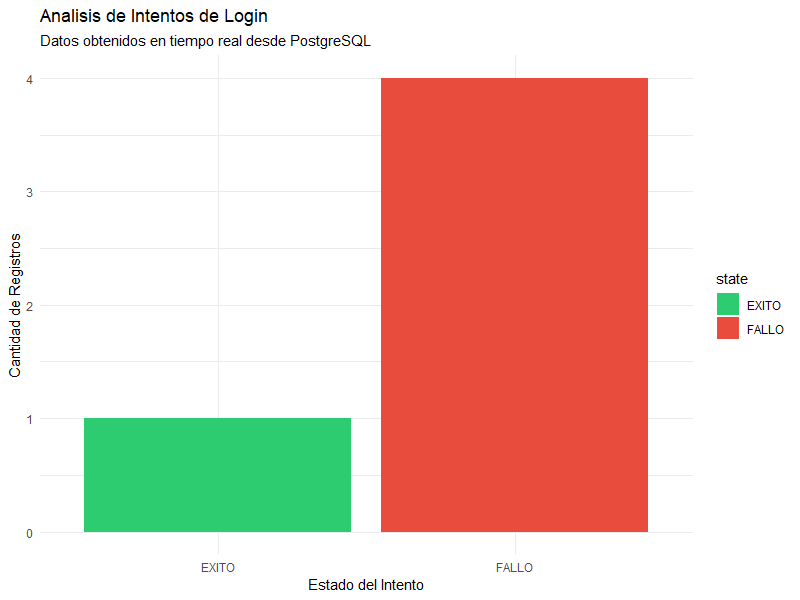
\includegraphics[width=0.8\textwidth]{reporte_auditoria.png}
    \caption{Distribución de intentos de login.}
\end{figure}

\section{Conclusión Técnica}
El sistema se encuentra operando bajo parámetros normales. Este reporte ha sido generado automáticamente por el servidor local.


\end{document}